% Saberes básicos (LOMLOE) asociados a esta unidad
%
% Bloque E. El cambio
%   - Interpretación macroscópica y microscópica de las reacciones químicas: explicación de las
%     relaciones de la química con el medio ambiente, la tecnología y la sociedad.
%     Justificación: se explica el mecanismo de una reacción química (choques efectivos entre
%     partículas) y se relacionan las reacciones químicas con la tecnología, el medio ambiente y
%     la sociedad (combustión, efecto invernadero, lluvia ácida, química verde).
%   - Ley de conservación de la masa y de la ley de las proporciones definidas: aplicación de
%     estas leyes como evidencias experimentales que permiten validar el modelo atómico-molecular
%     de la materia.
%     Justificación: se introduce la ley de conservación de la masa de Lavoisier y se aplica al
%     ajuste de ecuaciones químicas y a problemas numéricos con masas de reactivos y productos.
%   - Factores que afectan a las reacciones químicas: predicción cualitativa de la evolución de
%     las reacciones, entendiendo su importancia en la resolución de problemas actuales por parte
%     de la ciencia.
%     Justificación: se estudian la temperatura, la concentración, la superficie de contacto y
%     los catalizadores como factores que modifican la velocidad de una reacción, con ejemplos
%     cotidianos e industriales (motores, conservación de alimentos, enzimas...).
%
% (Traducción al español de Unit_6_Chemical_Reactions.tex. Unidad separada de la antigua
%  «Change of Matter»: los cambios físicos y químicos y la separación de mezclas están en la Unidad 5.)

\spacing{1.3}
\raggedbottom % las páginas con figuras grandes terminan donde acaba el texto

En la unidad anterior vimos que en un \textbf{cambio químico} aparecen sustancias nuevas. En esta unidad estudiaremos estos cambios con detalle: cómo tiene lugar una \textbf{reacción química}, cómo se escribe mediante una \textbf{ecuación química} y por qué \textbf{se conserva la masa}.

\section{Las reacciones químicas}

\begin{definition}[Reacción química]
    Proceso en el que unas sustancias, los \textbf{reactivos}, se transforman en otras sustancias nuevas, los \textbf{productos}.
\end{definition}

\subsection{¿Cómo tiene lugar una reacción química?}

\begin{enumerate}[label=\numberballmDarkTeal]
    \item Las partículas de los reactivos \textbf{chocan} entre sí.
    \item Si chocan con suficiente energía y con la orientación adecuada (un \textbf{choque eficaz}), se rompen los enlaces entre sus átomos.
    \item Los átomos se \textbf{reorganizan} y forman moléculas nuevas: los productos.
\end{enumerate}

\begin{figure}[H]
    \centering
    % [FIGURA ORIGINAL] \includegraphics[width=\textwidth]{Unit_6/collisions}
    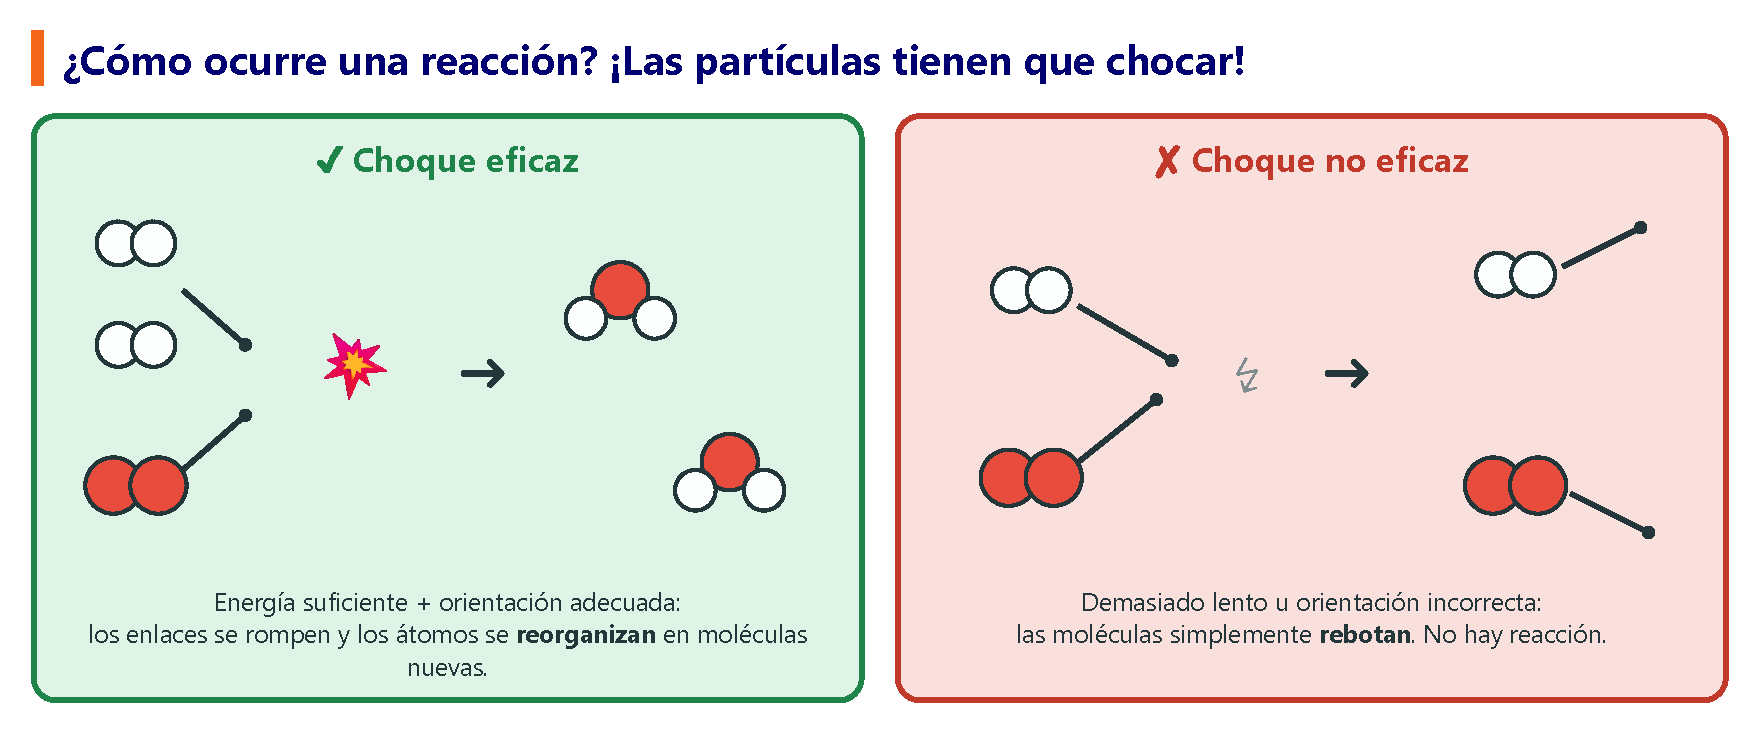
\includegraphics[width=\textwidth]{FigurasSVG/Unit_6_Chemical_Reactions/pdf/collisions_es.pdf}
    \caption{Solo los choques eficaces producen reacción: \(2\ch{H2} + \ch{O2} \longrightarrow 2\ch{H2O}\).}
    \label{fig:u6_collisions}
\end{figure}

\begin{exercise}
    Dentro de un recipiente hay moléculas de hidrógeno y de oxígeno. En el choque A, las moléculas se golpean muy suavemente; en el choque B, chocan deprisa y de frente. ¿En qué caso es más probable que haya reacción? ¿Por qué?
    \begin{solu}
        En el \textbf{choque B}. Un choque eficaz necesita \textbf{energía suficiente} y la orientación adecuada. En el choque A las moléculas chocan con demasiada suavidad, así que sus enlaces no se rompen y simplemente rebotan.
    \end{solu}
\end{exercise}

\begin{exercise}
    El agua oxigenada o peróxido de hidrógeno (\ch{H2O2}) se puede formar a partir de hidrógeno (\ch{H2}) y oxígeno (\ch{O2}).
    \begin{enumerate}[label=\letraminuscula]
        \item Identifica los reactivos y los productos.
        \item ¿Cuáles son sustancias simples y cuál es un compuesto?
    \end{enumerate}
    \begin{solu}
        \begin{enumerate}[label=\alph*)]
            \item Reactivos: \ch{H2} y \ch{O2}. Producto: \ch{H2O2}.
            \item \ch{H2} y \ch{O2} son \textbf{sustancias simples}; \ch{H2O2} es un \textbf{compuesto}.
        \end{enumerate}
    \end{solu}
\end{exercise}

\begin{exercise}
    ¿Verdadero o falso? Corrige las afirmaciones falsas.
    \begin{enumerate}[label=\letraminuscula]
        \item Todos los choques entre partículas de reactivos producen una reacción química.
        \item Un choque eficaz necesita energía suficiente y la orientación correcta.
        \item Los productos se forman cuando se rompen los enlaces de los reactivos y los átomos se reorganizan.
    \end{enumerate}
    \begin{solu}
        \begin{enumerate}[label=\alph*)]
            \item \textbf{Falso}: solo los choques \textit{eficaces} producen una reacción.
            \item \textbf{Verdadero}.
            \item \textbf{Verdadero}.
        \end{enumerate}
    \end{solu}
\end{exercise}

\subsection{Ecuaciones químicas y ley de conservación de la masa}

\begin{definition}[Ecuación química]
    Forma de escribir una reacción con fórmulas químicas: los reactivos a la izquierda, los productos a la derecha y una flecha entre ellos.
    \begin{equation*}
        \underbrace{\ch{N2} + 3\ch{H2}}_{\text{reactivos}} \longrightarrow \underbrace{2\ch{NH3}}_{\text{productos}}
    \end{equation*}
\end{definition}

\begin{figure}[H]
    \centering
    % [FIGURA ORIGINAL] \includegraphics[width=\textwidth]{Unit_6/conservation_mass}
    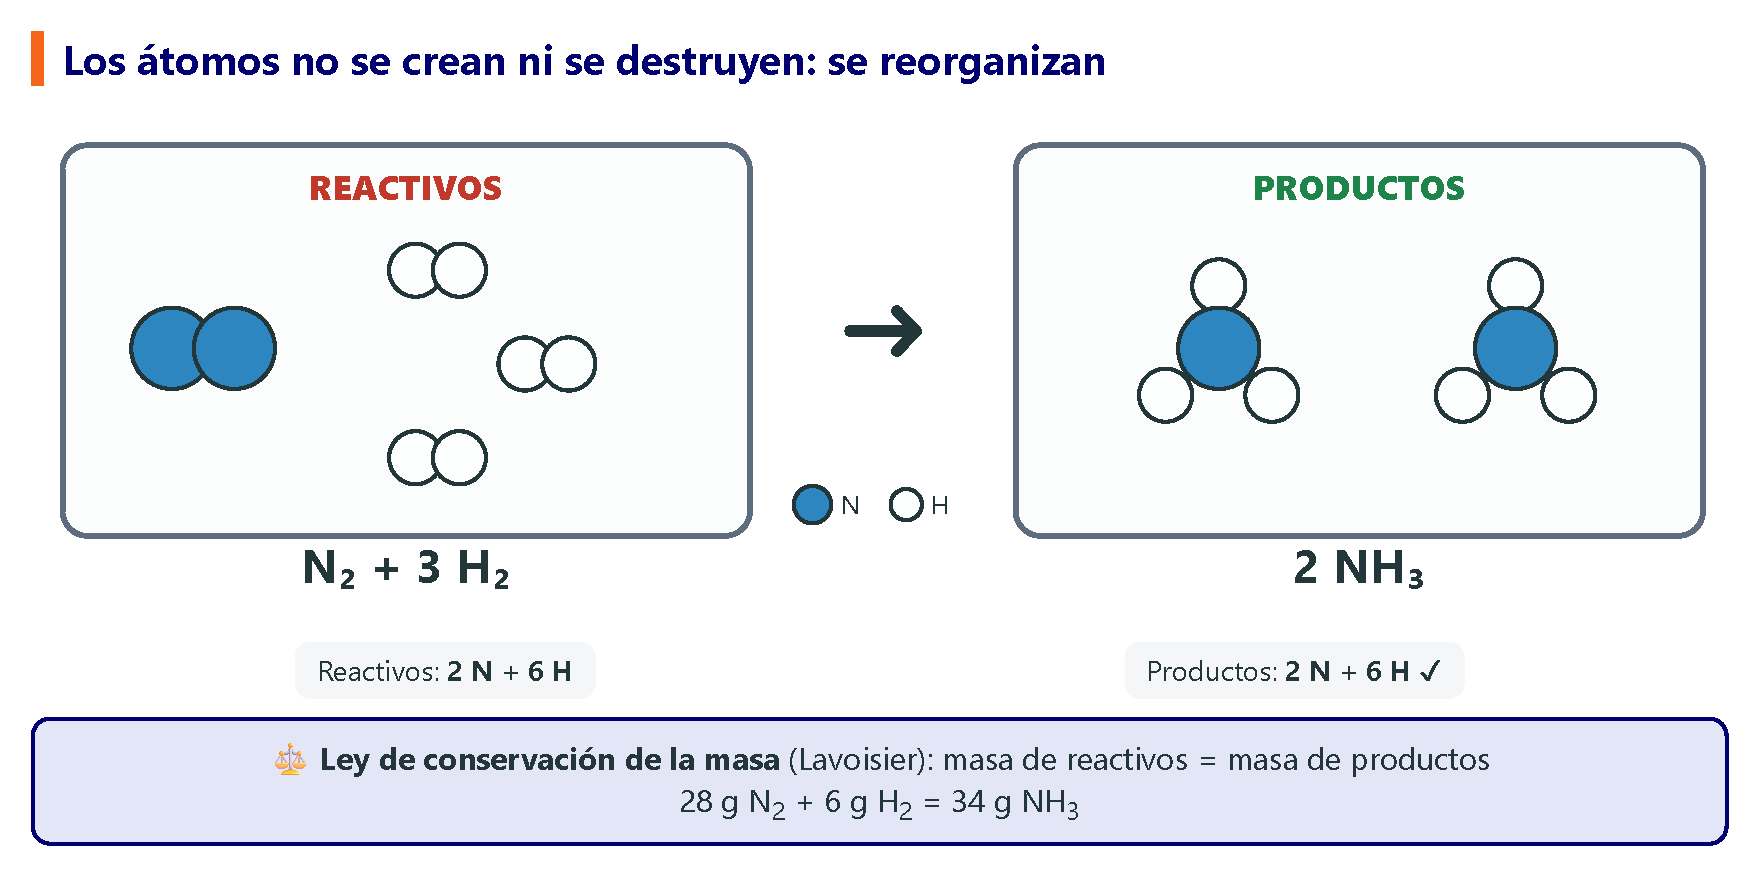
\includegraphics[width=\textwidth]{FigurasSVG/Unit_6_Chemical_Reactions/pdf/conservation_mass_es.pdf}
    \caption{Los mismos átomos antes y después: solo cambia la forma en que están unidos.}
    \label{fig:u6_conservation_mass}
\end{figure}

\begin{definition}[Ley de conservación de la masa]
    En una reacción química, la masa total de los reactivos es \textbf{igual} a la masa total de los productos. La materia no se crea ni se destruye, solo se transforma (Lavoisier, siglo \textsc{xviii}).
\end{definition}

\begin{didyouknow}
    Antoine Lavoisier, el «padre de la química moderna», pesaba todo con muchísimo cuidado en recipientes cerrados, y así descubrió la ley de conservación de la masa. Su famosa frase fue: «\emph{Nada se pierde, nada se crea, todo se transforma}».
\end{didyouknow}

\begin{example}
    \textbf{Ejemplo resuelto: uso de la ley de conservación de la masa paso a paso.} Cuando la piedra caliza (carbonato de calcio, \ch{CaCO3}) se calienta mucho, se descompone en cal viva (óxido de calcio, \ch{CaO}) y dióxido de carbono gaseoso (\ch{CO2}). Calentamos \qty{50}{\g} de carbonato de calcio en un recipiente cerrado hasta que reacciona todo y obtenemos \qty{28}{\g} de óxido de calcio. ¿Qué masa de dióxido de carbono se ha formado?
    \begin{enumerate}[label=\numberballmDarkTeal]
        \item \textbf{Identificamos los reactivos y los productos.} El reactivo es el carbonato de calcio; los productos son el óxido de calcio y el dióxido de carbono:
        \[
            \ch{CaCO3} \longrightarrow \ch{CaO} + \ch{CO2}
        \]
        \item \textbf{Anotamos los datos y la incógnita.} \(m(\ch{CaCO3}) = \qty{50}{\g}\); \quad \(m(\ch{CaO}) = \qty{28}{\g}\); \quad \(m(\ch{CO2}) = \ ?\)
        \item \textbf{Aplicamos la ley de conservación de la masa.} La masa total de los reactivos es igual a la masa total de los productos:
        \[
            m(\ch{CaCO3}) = m(\ch{CaO}) + m(\ch{CO2})
        \]
        \item \textbf{Sustituimos los datos.}
        \[
            \qty{50}{\g} = \qty{28}{\g} + m(\ch{CO2})
        \]
        \item \textbf{Despejamos la incógnita.} Los \qty{28}{\g} que están sumando a la derecha pasan a la izquierda restando:
        \[
            m(\ch{CO2}) = \qty{50}{\g} - \qty{28}{\g} = \textcolor{red}{\qty{22}{\g}}
        \]
        \item \textbf{Comprobamos el resultado.} Reactivos: \qty{50}{\g}. Productos: \(\qty{28}{\g} + \qty{22}{\g} = \qty{50}{\g}\). Las masas son iguales, así que la respuesta es correcta.
    \end{enumerate}
    \textbf{¿Por qué en un recipiente cerrado?} Si calentamos la caliza en un recipiente abierto, el \ch{CO2} se escapa al aire y al final la balanza solo marca \qty{28}{\g}: \emph{parece} que se han perdido \qty{22}{\g}. La masa no ha desaparecido; simplemente se ha ido en forma de gas. Por eso Lavoisier siempre pesaba sus reacciones en recipientes cerrados.
\end{example}

\begin{exercise}
    \qty{4}{\g} de hidrógeno reaccionan por completo con \qty{32}{\g} de oxígeno y forman agua. ¿Qué masa de agua se obtiene?
    \begin{solu}
        \(m(\ch{H2O}) = m(\ch{H2}) + m(\ch{O2}) = \qty{4}{\g} + \qty{32}{\g} = \qty{36}{\g}\).
    \end{solu}
\end{exercise}

\begin{exercise}
    \qty{5.6}{\g} de hierro reaccionan por completo con azufre y dan \qty{8.8}{\g} de sulfuro de hierro (\ch{FeS}). ¿Qué masa de azufre ha reaccionado?
    \begin{solu}
        \(m(\ch{S}) = m(\ch{FeS}) - m(\ch{Fe}) = \qty{8.8}{\g} - \qty{5.6}{\g} = \qty{3.2}{\g}\).
    \end{solu}
\end{exercise}

\begin{exercise}
    \qty{16}{\g} de metano (\ch{CH4}) arden por completo con \qty{64}{\g} de oxígeno y producen \qty{44}{\g} de dióxido de carbono y algo de vapor de agua. ¿Qué masa de vapor de agua se produce?
    \begin{solu}
        \(m(\ch{CH4}) + m(\ch{O2}) = m(\ch{CO2}) + m(\ch{H2O})\) \\
        \(\qty{16}{\g} + \qty{64}{\g} = \qty{44}{\g} + m(\ch{H2O}) \;\to\; m(\ch{H2O}) = \qty{36}{\g}\).
    \end{solu}
\end{exercise}

\subsection{Ajuste de ecuaciones químicas}

% Marcas para las tablas de ajuste: elemento ajustado / no ajustado
\providecommand{\balok}{\textcolor{green!50!black}{\(\checkmark\)}}
\providecommand{\balno}{\textcolor{red}{\(\boldsymbol{\times}\)}}

Ajustar una ecuación química es una de las destrezas más importantes de la química. En una reacción los átomos no se crean ni se destruyen (ley de conservación de la masa), así que la ecuación tiene que mostrar \textbf{los mismos átomos} antes y después de la reacción.

\begin{definition}[Ecuación química ajustada]
    Ecuación química que tiene el \textbf{mismo número de átomos de cada elemento} en el lado de los reactivos (izquierda) y en el de los productos (derecha).
\end{definition}

\begin{impt}
    \negsubro{Las tres reglas básicas}
    \begin{enumerate}[label=\numberballmDarkTeal]
        \item En los \textbf{reactivos} tiene que haber el \textbf{mismo número de átomos de cada elemento} que en los \textbf{productos}.
        \item \textbf{Contamos} los átomos de cada elemento, de uno en uno, en los reactivos (\textbf{izquierda}) y en los productos (\textbf{derecha}).
        \item Para que sea más fácil, es \textbf{conveniente} dejar el \textbf{hidrógeno} y el \textbf{oxígeno} para el \textbf{final}, y el oxígeno para el último de todos.
    \end{enumerate}
\end{impt}

\subsubsection{Coeficientes estequiométricos}

Para ajustar una ecuación solo podemos escribir números \textbf{delante} de las fórmulas. Estos números se llaman \negsubro{coeficientes estequiométricos}.

\begin{definition}[Coeficiente estequiométrico]
    Número entero (1, 2, 3\ldots) que se escribe \textbf{delante} de una fórmula en una ecuación química. \textbf{Multiplica} todos los átomos de esa fórmula. El coeficiente 1 no se escribe.
\end{definition}

\begin{figure}[H]
    \centering
    % [FIGURA ORIGINAL] \includegraphics[width=\textwidth]{Unit_6/coefficient_subscript}
    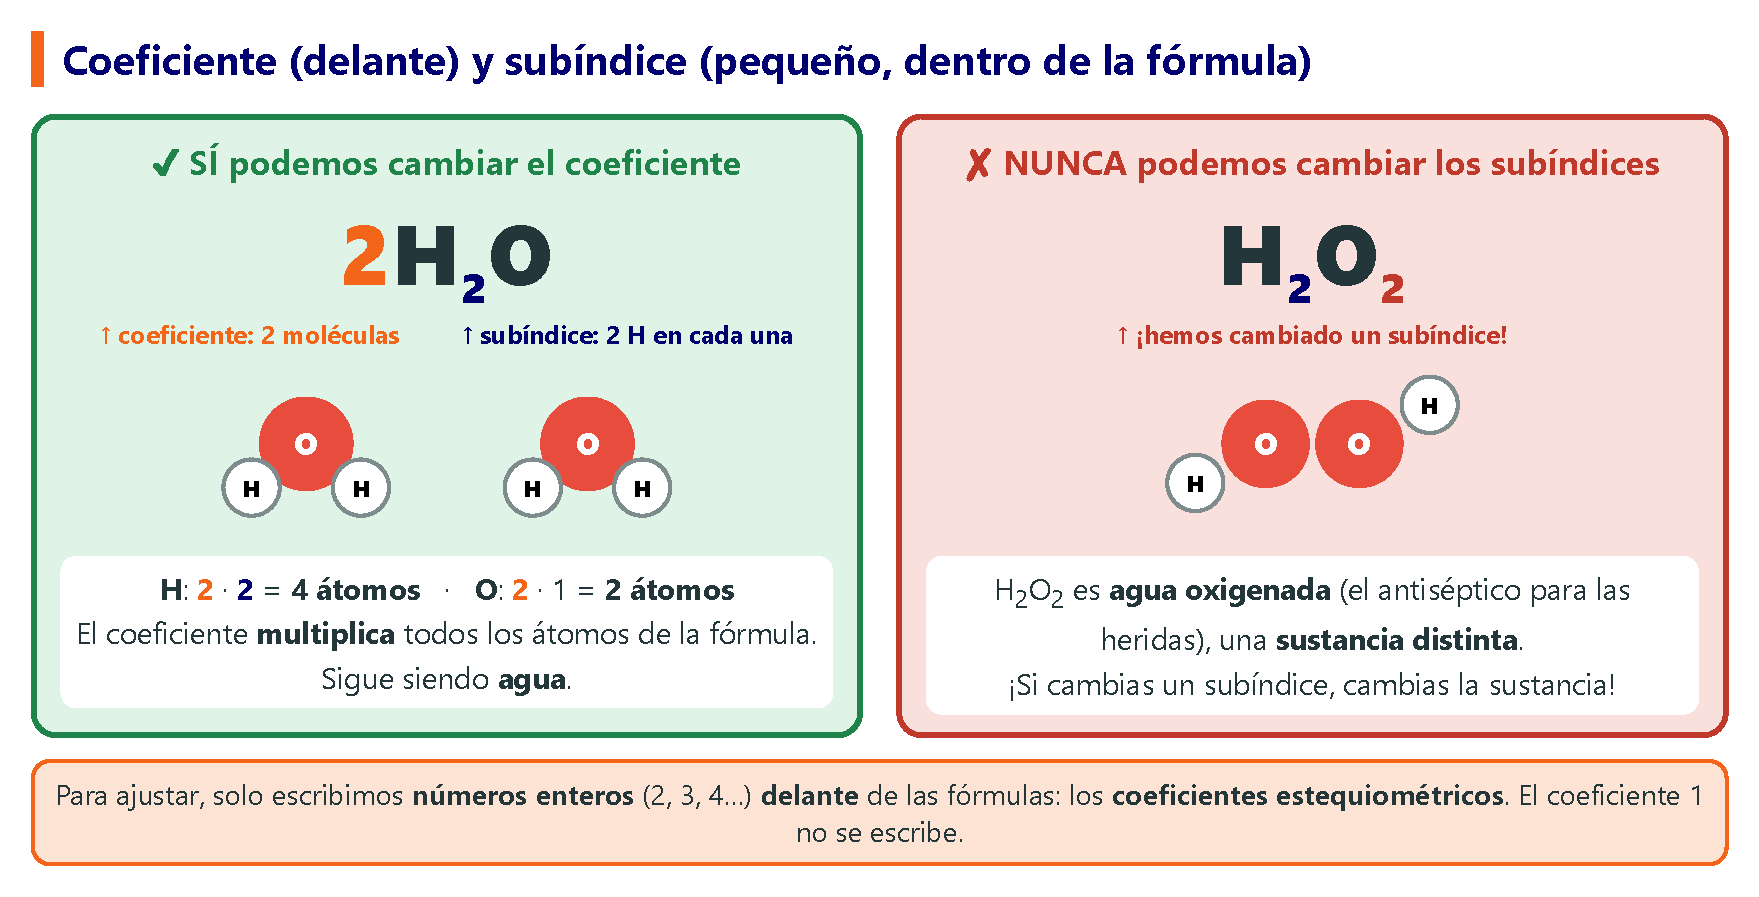
\includegraphics[width=\textwidth]{FigurasSVG/Unit_6_Chemical_Reactions/pdf/coefficient_subscript_es.pdf}
    \caption{El coeficiente multiplica toda la fórmula; los subíndices no se pueden cambiar nunca.}
    \label{fig:u6_coefficient_subscript}
\end{figure}

\begin{marker}
    \begin{itemize}
        \item Los coeficientes se escriben \textbf{delante} de la fórmula y \textbf{NUNCA como subíndice}. Si cambiamos un subíndice, cambiamos la sustancia: \ch{H2O} es agua, pero \ch{H2O2} es agua oxigenada (peróxido de hidrógeno).
        \item Al escribir un coeficiente, este \textbf{multiplica los subíndices} de todos los elementos de esa fórmula, así que cambia el número de átomos de \textbf{todos} los elementos de la fórmula: en \(3\ch{CO2}\) hay \(3 \cdot 1 = 3\) C y \(3 \cdot 2 = 6\) O.
        \item Los coeficientes tienen que ser siempre \textbf{números enteros}: 1, 2, 3\ldots{} (nunca \num{1.5} ni \(\frac{1}{2}\)).
    \end{itemize}
\end{marker}

\subsubsection{El método, paso a paso}

\begin{enumerate}[label=\numberballmDarkTeal]
    \item Escribe la ecuación y, \textbf{debajo, una tabla}: una fila para cada elemento y, bajo cada fórmula, el número de átomos de ese elemento. Añade una columna con el total de la izquierda y otra con el total de la derecha.
    \item Toma los elementos de uno en uno: primero los metales y los demás elementos, después el \textbf{hidrógeno} y por último el \textbf{oxígeno}.
    \item Para cada elemento, compara el total de la izquierda con el de la derecha:
    \begin{itemize}
        \item Si son \textbf{iguales}, el elemento está ajustado. \textbf{Mantenemos} los coeficientes y pasamos al siguiente elemento.
        \item Si son \textbf{distintos}, vamos al lado que tiene \textbf{menos} átomos de ese elemento y escribimos delante de la fórmula que lo contiene un coeficiente \textbf{una unidad mayor} (si no hay número, es un 1, así que escribimos un 2). \textbf{Volvemos a contar}. Si los dos lados siguen siendo distintos, aumentamos otra vez en uno el coeficiente del lado que \textbf{ahora} tiene menos átomos, y repetimos hasta que los dos lados sean iguales.
    \end{itemize}
    \item \textbf{Cuidado}: al escribir un coeficiente, también cambian los demás elementos de esa fórmula. Por eso, cada vez que ajustamos un elemento nuevo, hay que \textbf{comprobar de nuevo} que los elementos que ya estaban ajustados lo siguen estando. Si alguno no lo está, lo volvemos a ajustar.
    \item Cuando \textbf{todos} los elementos están ajustados, la ecuación está ajustada. Si todos los coeficientes se pueden dividir por un mismo número, los simplificamos (\(2, 4, 2 \to 1, 2, 1\)).
\end{enumerate}

\begin{figure}[H]
    \centering
    % [FIGURA ORIGINAL] \includegraphics[width=0.95\textwidth]{Unit_6/balancing_method}
    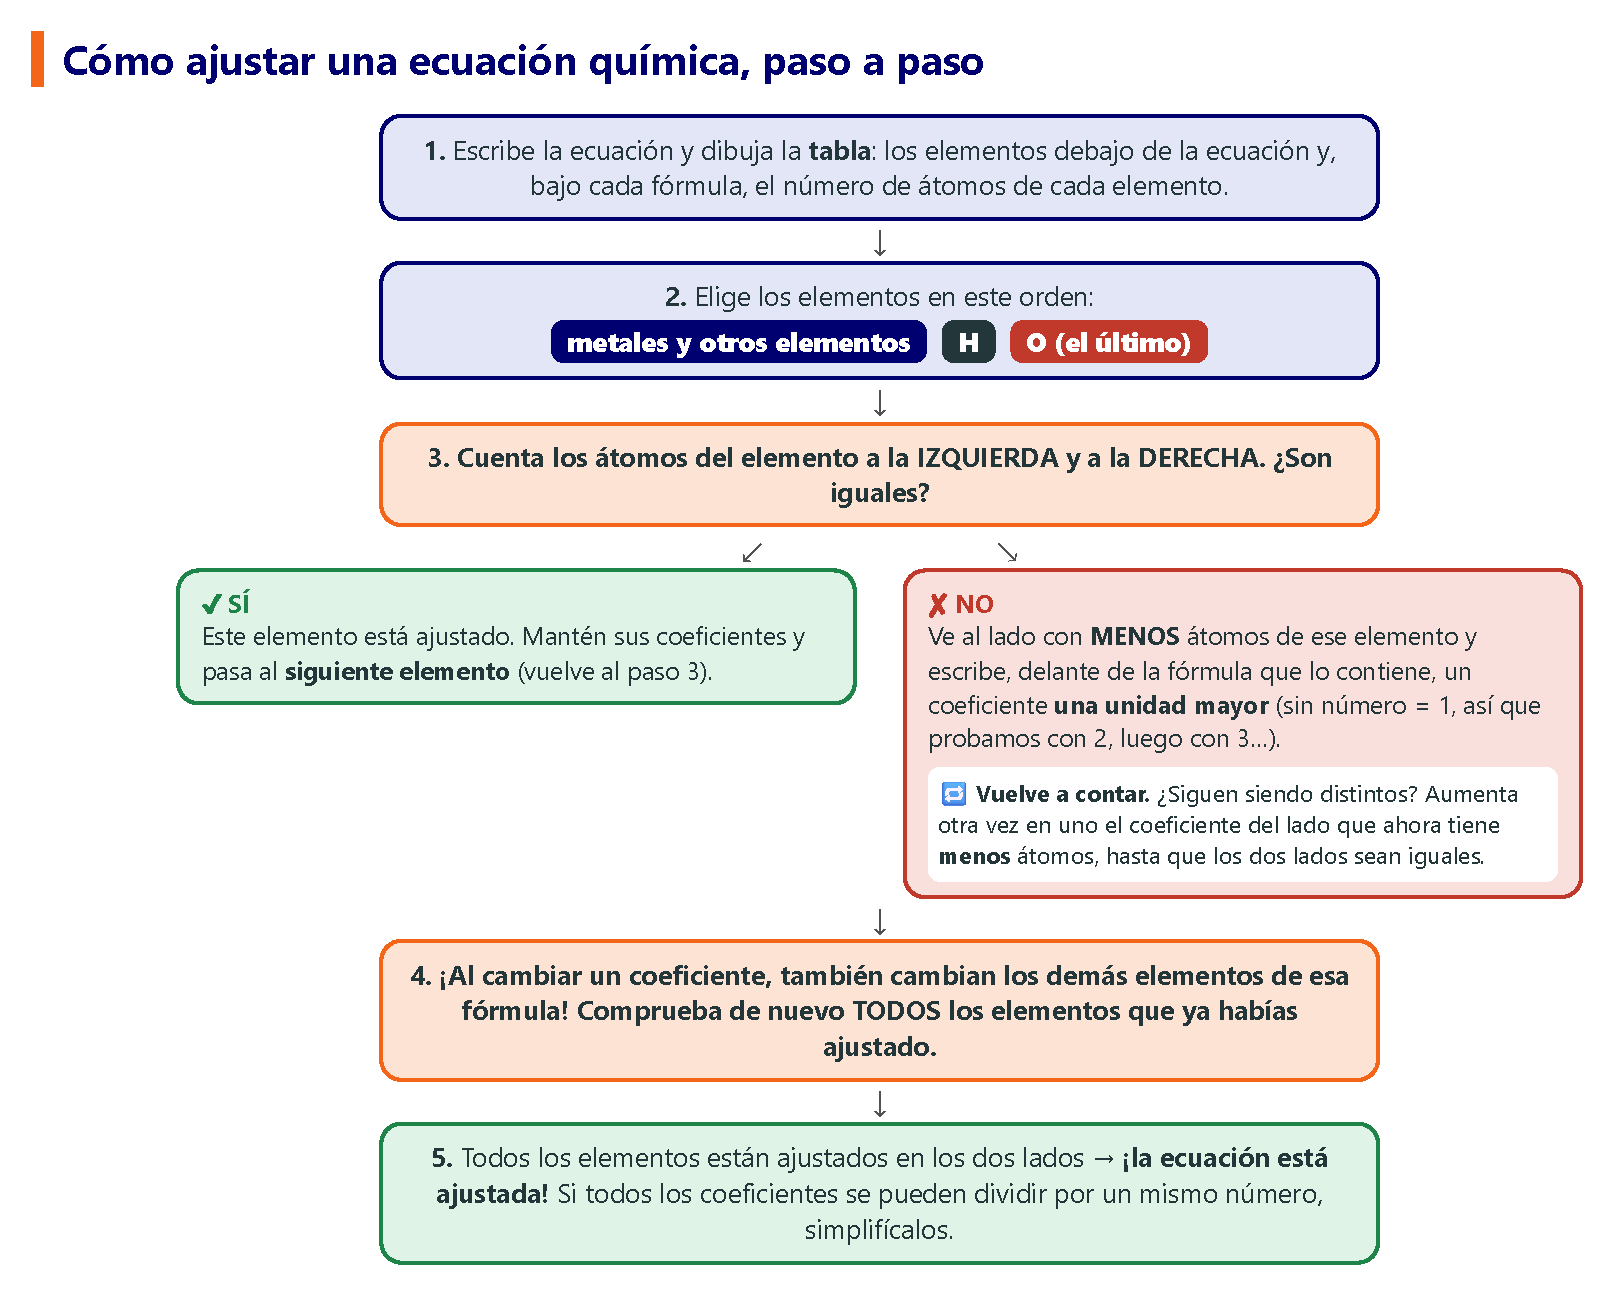
\includegraphics[width=0.95\textwidth]{FigurasSVG/Unit_6_Chemical_Reactions/pdf/balancing_method_es.pdf}
    \caption{El método para ajustar una ecuación química.}
    \label{fig:u6_balancing_method}
\end{figure}

\begin{impt}
    \negsubro{La tabla de ajuste}: debajo de la ecuación escribimos los elementos y, bajo cada fórmula, el número de átomos de cada elemento. Cuando una fórmula lleva coeficiente, multiplicamos: coeficiente \(\cdot\) subíndice. Las columnas \textbf{Izquierda} y \textbf{Derecha} muestran los totales, y la última columna nos dice si ese elemento está ajustado (\balok) o no (\balno). La fila del elemento con el que estamos trabajando está \colorbox{yellow!25}{resaltada}, y el coeficiente que acabamos de escribir aparece en \textcolor{red}{\textbf{rojo}}.
\end{impt}

\begin{example}
    \textbf{Ajusta la ecuación de formación del amoniaco: } \(\ch{N2} + \ch{H2} \longrightarrow \ch{NH3}\)
\end{example}

\negsubro{Paso 1}: dibujamos la tabla y contamos los átomos de cada elemento.
\begin{center}
    \small\renewcommand{\arraystretch}{1.3}
    % --- tabla antigua ---
    % \begin{tabular}{l|cc|>{\columncolor{blue!8}}c||c|>{\columncolor{blue!8}}c|c}
        % \textbf{Element} & \ch{N2} & \ch{H2} & \textbf{Left} & \ch{NH3} & \textbf{Right} &  \\
        % \hline
        % \textbf{N} & 2 & -- & \textbf{2} & 1 & \textbf{1} & \balno \\
        % \textbf{H} & -- & 2 & \textbf{2} & 3 & \textbf{3} & \balno \\
    % \end{tabular}
    % --- tabla nueva ---
    \begin{tabular}{@{}lcccccc@{}}
        \toprule
        \textbf{Elemento} & \textbf{\ch{N2}} & \textbf{\ch{H2}} & \textbf{Izquierda} & \textbf{\ch{NH3}} & \textbf{Derecha} &  \\
        \midrule
        \textbf{N} & 2 & -- & \textbf{2} & 1 & \textbf{1} & \balno \\[3pt]
        \textbf{H} & -- & 2 & \textbf{2} & 3 & \textbf{3} & \balno \\
        \bottomrule
    \end{tabular}
\end{center}

\negsubro{Paso 2: nitrógeno.} A la izquierda hay 2 N y a la derecha solo 1 N. El lado \textbf{derecho} tiene menos, así que escribimos un \textbf{2} delante de \ch{NH3}. Volvemos a contar: \(2 \cdot 1 = 2\) N a la derecha. \balok{} Fíjate en que los H de la derecha también han cambiado: \(2 \cdot 3 = 6\).
\begin{center}
    \small\renewcommand{\arraystretch}{1.3}
    % --- tabla antigua ---
    % \begin{tabular}{l|cc|>{\columncolor{blue!8}}c||c|>{\columncolor{blue!8}}c|c}
        % \textbf{Element} & \ch{N2} & \ch{H2} & \textbf{Left} & \textcolor{red}{\textbf{2}}\ch{NH3} & \textbf{Right} &  \\
        % \hline
        % \rowcolor{yellow!25} \textbf{N} & 2 & -- & \textbf{2} & \(2 \cdot 1 = 2\) & \textbf{2} & \balok \\
        % \textbf{H} & -- & 2 & \textbf{2} & \(2 \cdot 3 = 6\) & \textbf{6} & \balno \\
    % \end{tabular}
    % --- tabla nueva ---
    \begin{tabular}{@{}lcccccc@{}}
        \toprule
        \textbf{Elemento} & \textbf{\ch{N2}} & \textbf{\ch{H2}} & \textbf{Izquierda} & \textcolor{red}{\textbf{2}}\ch{NH3} & \textbf{Derecha} &  \\
        \midrule
        \textbf{N} & 2 & -- & \textbf{2} & \(2 \cdot 1 = 2\) & \textbf{2} & \balok \\[3pt]
        \textbf{H} & -- & 2 & \textbf{2} & \(2 \cdot 3 = 6\) & \textbf{6} & \balno \\
        \bottomrule
    \end{tabular}
\end{center}
\negsubro{Paso 3: hidrógeno.} A la izquierda hay 2 H y a la derecha 6 H. El lado \textbf{izquierdo} tiene menos, así que aumentamos el coeficiente de \ch{H2} de uno en uno: con un 2 tenemos \(2 \cdot 2 = 4\) H \balno; con un 3 tenemos \(3 \cdot 2 = 6\) H \balok.
\begin{center}
    \small\renewcommand{\arraystretch}{1.3}
    % --- tabla antigua ---
    % \begin{tabular}{l|cc|>{\columncolor{blue!8}}c||c|>{\columncolor{blue!8}}c|c}
        % \textbf{Element} & \ch{N2} & \textcolor{red}{\textbf{3}}\ch{H2} & \textbf{Left} & 2\ch{NH3} & \textbf{Right} &  \\
        % \hline
        % \textbf{N} & 2 & -- & \textbf{2} & \(2 \cdot 1 = 2\) & \textbf{2} & \balok \\
        % \rowcolor{yellow!25} \textbf{H} & -- & \(3 \cdot 2 = 6\) & \textbf{6} & \(2 \cdot 3 = 6\) & \textbf{6} & \balok \\
    % \end{tabular}
    % --- tabla nueva ---
    \begin{tabular}{@{}lcccccc@{}}
        \toprule
        \textbf{Elemento} & \textbf{\ch{N2}} & \textcolor{red}{\textbf{3}}\ch{H2} & \textbf{Izquierda} & \textbf{2\ch{NH3}} & \textbf{Derecha} &  \\
        \midrule
        \textbf{N} & 2 & -- & \textbf{2} & \(2 \cdot 1 = 2\) & \textbf{2} & \balok \\[3pt]
        \textbf{H} & -- & \(3 \cdot 2 = 6\) & \textbf{6} & \(2 \cdot 3 = 6\) & \textbf{6} & \balok \\
        \bottomrule
    \end{tabular}
\end{center}
\negsubro{Paso 4: comprobación.} El nitrógeno sigue ajustado (2 = 2) y el hidrógeno también (6 = 6). La ecuación ajustada es:
\begin{equation*}
    \ch{N2} + 3\ch{H2} \longrightarrow 2\ch{NH3}
\end{equation*}

\begin{example}
    \textbf{Ajusta la combustión del metano (gas natural): } \(\ch{CH4} + \ch{O2} \longrightarrow \ch{CO2} + \ch{H2O}\)
\end{example}

\negsubro{Paso 1}: la tabla. Dejaremos el H y el O para el final, y el O para el último de todos.
\begin{center}
    \small\renewcommand{\arraystretch}{1.3}
    % --- tabla antigua ---
    % \begin{tabular}{l|cc|>{\columncolor{blue!8}}c||cc|>{\columncolor{blue!8}}c|c}
        % \textbf{Element} & \ch{CH4} & \ch{O2} & \textbf{Left} & \ch{CO2} & \ch{H2O} & \textbf{Right} &  \\
        % \hline
        % \textbf{C} & 1 & -- & \textbf{1} & 1 & -- & \textbf{1} & \balok \\
        % \textbf{H} & 4 & -- & \textbf{4} & -- & 2 & \textbf{2} & \balno \\
        % \textbf{O} & -- & 2 & \textbf{2} & 2 & 1 & \textbf{3} & \balno \\
    % \end{tabular}
    % --- tabla nueva ---
    \begin{tabular}{@{}lccccccc@{}}
        \toprule
        \textbf{Elemento} & \textbf{\ch{CH4}} & \textbf{\ch{O2}} & \textbf{Izquierda} & \textbf{\ch{CO2}} & \textbf{\ch{H2O}} & \textbf{Derecha} &  \\
        \midrule
        \textbf{C} & 1 & -- & \textbf{1} & 1 & -- & \textbf{1} & \balok \\[3pt]
        \textbf{H} & 4 & -- & \textbf{4} & -- & 2 & \textbf{2} & \balno \\[3pt]
        \textbf{O} & -- & 2 & \textbf{2} & 2 & 1 & \textbf{3} & \balno \\
        \bottomrule
    \end{tabular}
\end{center}

\negsubro{Paso 2: carbono.} 1 C a la izquierda y 1 C a la derecha. \balok{} Pasamos al siguiente elemento.

\negsubro{Paso 3: hidrógeno.} 4 H a la izquierda y 2 H a la derecha. El lado \textbf{derecho} tiene menos, así que escribimos un \textbf{2} delante de \ch{H2O}: \(2 \cdot 2 = 4\) H. \balok
\begin{center}
    \small\renewcommand{\arraystretch}{1.3}
    % --- tabla antigua ---
    % \begin{tabular}{l|cc|>{\columncolor{blue!8}}c||cc|>{\columncolor{blue!8}}c|c}
        % \textbf{Element} & \ch{CH4} & \ch{O2} & \textbf{Left} & \ch{CO2} & \textcolor{red}{\textbf{2}}\ch{H2O} & \textbf{Right} &  \\
        % \hline
        % \textbf{C} & 1 & -- & \textbf{1} & 1 & -- & \textbf{1} & \balok \\
        % \rowcolor{yellow!25} \textbf{H} & 4 & -- & \textbf{4} & -- & \(2 \cdot 2 = 4\) & \textbf{4} & \balok \\
        % \textbf{O} & -- & 2 & \textbf{2} & 2 & \(2 \cdot 1 = 2\) & \textbf{4} & \balno \\
    % \end{tabular}
    % --- tabla nueva ---
    \begin{tabular}{@{}lccccccc@{}}
        \toprule
        \textbf{Elemento} & \textbf{\ch{CH4}} & \textbf{\ch{O2}} & \textbf{Izquierda} & \textbf{\ch{CO2}} & \textcolor{red}{\textbf{2}}\ch{H2O} & \textbf{Derecha} &  \\
        \midrule
        \textbf{C} & 1 & -- & \textbf{1} & 1 & -- & \textbf{1} & \balok \\[3pt]
        \textbf{H} & 4 & -- & \textbf{4} & -- & \(2 \cdot 2 = 4\) & \textbf{4} & \balok \\[3pt]
        \textbf{O} & -- & 2 & \textbf{2} & 2 & \(2 \cdot 1 = 2\) & \textbf{4} & \balno \\
        \bottomrule
    \end{tabular}
\end{center}
\negsubro{Paso 4: oxígeno (el último).} A la izquierda hay 2 O; a la derecha, \(2 + 2 = 4\) O (2 en el \ch{CO2} y 2 en \(2\ch{H2O}\)). El lado \textbf{izquierdo} tiene menos, así que escribimos un \textbf{2} delante de \ch{O2}: \(2 \cdot 2 = 4\) O. \balok
\begin{center}
    \small\renewcommand{\arraystretch}{1.3}
    % --- tabla antigua ---
    % \begin{tabular}{l|cc|>{\columncolor{blue!8}}c||cc|>{\columncolor{blue!8}}c|c}
        % \textbf{Element} & \ch{CH4} & \textcolor{red}{\textbf{2}}\ch{O2} & \textbf{Left} & \ch{CO2} & 2\ch{H2O} & \textbf{Right} &  \\
        % \hline
        % \textbf{C} & 1 & -- & \textbf{1} & 1 & -- & \textbf{1} & \balok \\
        % \textbf{H} & 4 & -- & \textbf{4} & -- & \(2 \cdot 2 = 4\) & \textbf{4} & \balok \\
        % \rowcolor{yellow!25} \textbf{O} & -- & \(2 \cdot 2 = 4\) & \textbf{4} & 2 & \(2 \cdot 1 = 2\) & \textbf{4} & \balok \\
    % \end{tabular}
    % --- tabla nueva ---
    \begin{tabular}{@{}lccccccc@{}}
        \toprule
        \textbf{Elemento} & \textbf{\ch{CH4}} & \textcolor{red}{\textbf{2}}\ch{O2} & \textbf{Izquierda} & \textbf{\ch{CO2}} & \textbf{2\ch{H2O}} & \textbf{Derecha} &  \\
        \midrule
        \textbf{C} & 1 & -- & \textbf{1} & 1 & -- & \textbf{1} & \balok \\[3pt]
        \textbf{H} & 4 & -- & \textbf{4} & -- & \(2 \cdot 2 = 4\) & \textbf{4} & \balok \\[3pt]
        \textbf{O} & -- & \(2 \cdot 2 = 4\) & \textbf{4} & 2 & \(2 \cdot 1 = 2\) & \textbf{4} & \balok \\
        \bottomrule
    \end{tabular}
\end{center}
\negsubro{Paso 5: comprobación.} C: 1 = 1; H: 4 = 4; O: 4 = 4. La ecuación ajustada es:
\begin{equation*}
    \ch{CH4} + 2\ch{O2} \longrightarrow \ch{CO2} + 2\ch{H2O}
\end{equation*}
Dejar el oxígeno para el final lo ha hecho fácil: el \ch{O2} solo contiene oxígeno, así que al cambiar su coeficiente no se ha desajustado ningún otro elemento.

\begin{example}
    \textbf{Ajusta la oxidación del aluminio: } \(\ch{Al} + \ch{O2} \longrightarrow \ch{Al2O3}\) \textbf{(un caso más difícil)}
\end{example}

\negsubro{Paso 1}: la tabla.
\begin{center}
    \small\renewcommand{\arraystretch}{1.3}
    % --- tabla antigua ---
    % \begin{tabular}{l|cc|>{\columncolor{blue!8}}c||c|>{\columncolor{blue!8}}c|c}
        % \textbf{Element} & \ch{Al} & \ch{O2} & \textbf{Left} & \ch{Al2O3} & \textbf{Right} &  \\
        % \hline
        % \textbf{Al} & 1 & -- & \textbf{1} & 2 & \textbf{2} & \balno \\
        % \textbf{O} & -- & 2 & \textbf{2} & 3 & \textbf{3} & \balno \\
    % \end{tabular}
    % --- tabla nueva ---
    \begin{tabular}{@{}lcccccc@{}}
        \toprule
        \textbf{Elemento} & \textbf{\ch{Al}} & \textbf{\ch{O2}} & \textbf{Izquierda} & \textbf{\ch{Al2O3}} & \textbf{Derecha} &  \\
        \midrule
        \textbf{Al} & 1 & -- & \textbf{1} & 2 & \textbf{2} & \balno \\[3pt]
        \textbf{O} & -- & 2 & \textbf{2} & 3 & \textbf{3} & \balno \\
        \bottomrule
    \end{tabular}
\end{center}

\negsubro{Paso 2: aluminio.} 1 Al a la izquierda y 2 Al a la derecha. El lado \textbf{izquierdo} tiene menos: escribimos un \textbf{2} delante de \ch{Al}. \balok
\begin{center}
    \small\renewcommand{\arraystretch}{1.3}
    % --- tabla antigua ---
    % \begin{tabular}{l|cc|>{\columncolor{blue!8}}c||c|>{\columncolor{blue!8}}c|c}
        % \textbf{Element} & \textcolor{red}{\textbf{2}}\ch{Al} & \ch{O2} & \textbf{Left} & \ch{Al2O3} & \textbf{Right} &  \\
        % \hline
        % \rowcolor{yellow!25} \textbf{Al} & \(2 \cdot 1 = 2\) & -- & \textbf{2} & 2 & \textbf{2} & \balok \\
        % \textbf{O} & -- & 2 & \textbf{2} & 3 & \textbf{3} & \balno \\
    % \end{tabular}
    % --- tabla nueva ---
    \begin{tabular}{@{}lcccccc@{}}
        \toprule
        \textbf{Elemento} & \textcolor{red}{\textbf{2}}\ch{Al} & \textbf{\ch{O2}} & \textbf{Izquierda} & \textbf{\ch{Al2O3}} & \textbf{Derecha} &  \\
        \midrule
        \textbf{Al} & \(2 \cdot 1 = 2\) & -- & \textbf{2} & 2 & \textbf{2} & \balok \\[3pt]
        \textbf{O} & -- & 2 & \textbf{2} & 3 & \textbf{3} & \balno \\
        \bottomrule
    \end{tabular}
\end{center}
\negsubro{Paso 3: oxígeno.} 2 O a la izquierda y 3 O a la derecha. Cada vez, aumentamos en uno el coeficiente del lado que tiene \textbf{menos} átomos en ese momento:
\begin{itemize}
    \item La izquierda tiene menos (\(2 < 3\)): \(2\ch{O2}\) \(\to\) 4 O a la izquierda. Ahora \(4 > 3\) \balno
    \item Ahora la derecha tiene menos (\(3 < 4\)): \(2\ch{Al2O3}\) \(\to\) \(2 \cdot 3 = 6\) O a la derecha. \(4 < 6\) \balno
    \item La izquierda vuelve a tener menos (\(4 < 6\)): \(3\ch{O2}\) \(\to\) \(3 \cdot 2 = 6\) O. \(6 = 6\) \balok
\end{itemize}
\begin{center}
    \small\renewcommand{\arraystretch}{1.3}
    % --- tabla antigua ---
    % \begin{tabular}{l|cc|>{\columncolor{blue!8}}c||c|>{\columncolor{blue!8}}c|c}
        % \textbf{Element} & 2\ch{Al} & \textcolor{red}{\textbf{3}}\ch{O2} & \textbf{Left} & 2\ch{Al2O3} & \textbf{Right} &  \\
        % \hline
        % \textbf{Al} & \(2 \cdot 1 = 2\) & -- & \textbf{2} & \(2 \cdot 2 = 4\) & \textbf{4} & \balno \\
        % \rowcolor{yellow!25} \textbf{O} & -- & \(3 \cdot 2 = 6\) & \textbf{6} & \(2 \cdot 3 = 6\) & \textbf{6} & \balok \\
    % \end{tabular}
    % --- tabla nueva ---
    \begin{tabular}{@{}lcccccc@{}}
        \toprule
        \textbf{Elemento} & \textbf{2\ch{Al}} & \textcolor{red}{\textbf{3}}\ch{O2} & \textbf{Izquierda} & \textbf{2\ch{Al2O3}} & \textbf{Derecha} &  \\
        \midrule
        \textbf{Al} & \(2 \cdot 1 = 2\) & -- & \textbf{2} & \(2 \cdot 2 = 4\) & \textbf{4} & \balno \\[3pt]
        \textbf{O} & -- & \(3 \cdot 2 = 6\) & \textbf{6} & \(2 \cdot 3 = 6\) & \textbf{6} & \balok \\
        \bottomrule
    \end{tabular}
\end{center}
\negsubro{Paso 4: ¡comprueba los elementos que ya estaban ajustados!} Al escribir el 2 delante de \ch{Al2O3}, cambió el aluminio de la derecha: ahora hay \(2 \cdot 2 = 4\) Al a la derecha, pero solo 2 a la izquierda. \balno{} La izquierda tiene menos: probamos con \(3\ch{Al}\) (3 Al \balno) y después con \(4\ch{Al}\) (4 Al \balok).
\begin{center}
    \small\renewcommand{\arraystretch}{1.3}
    % --- tabla antigua ---
    % \begin{tabular}{l|cc|>{\columncolor{blue!8}}c||c|>{\columncolor{blue!8}}c|c}
        % \textbf{Element} & \textcolor{red}{\textbf{4}}\ch{Al} & 3\ch{O2} & \textbf{Left} & 2\ch{Al2O3} & \textbf{Right} &  \\
        % \hline
        % \rowcolor{yellow!25} \textbf{Al} & \(4 \cdot 1 = 4\) & -- & \textbf{4} & \(2 \cdot 2 = 4\) & \textbf{4} & \balok \\
        % \textbf{O} & -- & \(3 \cdot 2 = 6\) & \textbf{6} & \(2 \cdot 3 = 6\) & \textbf{6} & \balok \\
    % \end{tabular}
    % --- tabla nueva ---
    \begin{tabular}{@{}lcccccc@{}}
        \toprule
        \textbf{Elemento} & \textcolor{red}{\textbf{4}}\ch{Al} & \textbf{3\ch{O2}} & \textbf{Izquierda} & \textbf{2\ch{Al2O3}} & \textbf{Derecha} &  \\
        \midrule
        \textbf{Al} & \(4 \cdot 1 = 4\) & -- & \textbf{4} & \(2 \cdot 2 = 4\) & \textbf{4} & \balok \\[3pt]
        \textbf{O} & -- & \(3 \cdot 2 = 6\) & \textbf{6} & \(2 \cdot 3 = 6\) & \textbf{6} & \balok \\
        \bottomrule
    \end{tabular}
\end{center}
\negsubro{Paso 5: comprobación final.} Al: 4 = 4; O: 6 = 6. La ecuación ajustada es:
\begin{equation*}
    4\ch{Al} + 3\ch{O2} \longrightarrow 2\ch{Al2O3}
\end{equation*}

\begin{exercise}
    Ajusta estas ecuaciones químicas:
    \begin{enumerate}[label=\letraminuscula]
        \item \(\ch{Mg} + \ch{O2} \longrightarrow \ch{MgO}\)
        \item \(\ch{Fe} + \ch{HCl} \longrightarrow \ch{FeCl2} + \ch{H2}\)
        \item \(\ch{C3H8} + \ch{O2} \longrightarrow \ch{CO2} + \ch{H2O}\)
    \end{enumerate}
    \begin{solu}
        \begin{enumerate}[label=\alph*)]
            \item \(2\ch{Mg} + \ch{O2} \longrightarrow 2\ch{MgO}\)
            \item \(\ch{Fe} + 2\ch{HCl} \longrightarrow \ch{FeCl2} + \ch{H2}\)
            \item \(\ch{C3H8} + 5\ch{O2} \longrightarrow 3\ch{CO2} + 4\ch{H2O}\)
        \end{enumerate}
    \end{solu}
\end{exercise}

\begin{exercise}
    Ajusta estas ecuaciones químicas:
    \begin{enumerate}[label=\letraminuscula]
        \item \(\ch{Al} + \ch{O2} \longrightarrow \ch{Al2O3}\)
        \item \(\ch{CH4} + \ch{O2} \longrightarrow \ch{CO2} + \ch{H2O}\)
        \item \(\ch{Na} + \ch{Cl2} \longrightarrow \ch{NaCl}\)
    \end{enumerate}
    \begin{solu}
        \begin{enumerate}[label=\alph*)]
            \item \(4\ch{Al} + 3\ch{O2} \longrightarrow 2\ch{Al2O3}\)
            \item \(\ch{CH4} + 2\ch{O2} \longrightarrow \ch{CO2} + 2\ch{H2O}\)
            \item \(2\ch{Na} + \ch{Cl2} \longrightarrow 2\ch{NaCl}\)
        \end{enumerate}
    \end{solu}
\end{exercise}

\begin{exercise}
    Ajusta estas ecuaciones químicas usando la tabla de ajuste:
    \begin{enumerate}[label=\letraminuscula]
        \item \(\ch{H2} + \ch{O2} \longrightarrow \ch{H2O}\)
        \item \(\ch{Zn} + \ch{HCl} \longrightarrow \ch{ZnCl2} + \ch{H2}\)
        \item \(\ch{KClO3} \longrightarrow \ch{KCl} + \ch{O2}\)
        \item \(\ch{Fe} + \ch{O2} \longrightarrow \ch{Fe2O3}\)
        \item \(\ch{C2H4} + \ch{O2} \longrightarrow \ch{CO2} + \ch{H2O}\)
    \end{enumerate}
    \begin{solu}
        \begin{enumerate}[label=\alph*)]
            \item \(2\ch{H2} + \ch{O2} \longrightarrow 2\ch{H2O}\)
            \item \(\ch{Zn} + 2\ch{HCl} \longrightarrow \ch{ZnCl2} + \ch{H2}\)
            \item \(2\ch{KClO3} \longrightarrow 2\ch{KCl} + 3\ch{O2}\)
            \item \(4\ch{Fe} + 3\ch{O2} \longrightarrow 2\ch{Fe2O3}\)
            \item \(\ch{C2H4} + 3\ch{O2} \longrightarrow 2\ch{CO2} + 2\ch{H2O}\)
        \end{enumerate}
    \end{solu}
\end{exercise}

% (Las secciones comentadas de la versión inglesa —Important chemical reactions, Chemical reactions,
%  technology and society, How to change the speed of a reaction— no se han traducido porque no se
%  compilan; están en Unit_6_Chemical_Reactions.tex.)

%----------------------------------------------------------------------------------------

\section*{Resumen}

\begin{itemize}
    \item \textbf{Reacción química}: reactivos \(\to\) productos. Ocurre mediante \textbf{choques eficaces}: se rompen enlaces y los átomos se reorganizan.
    \item Las \textbf{ecuaciones químicas} se tienen que \textbf{ajustar} con coeficientes (nunca se cambian los subíndices).
    \item \textbf{Ley de conservación de la masa} (Lavoisier): masa de reactivos = masa de productos.
\end{itemize}

\section{Vocabulario}

\begin{vocabulary}[Reactivo (\textit{reactant})]
    Sustancia que reacciona en una reacción química.
\end{vocabulary}

\begin{vocabulary}[Producto (\textit{product})]
    Sustancia que se obtiene en una reacción química.
\end{vocabulary}

\begin{vocabulary}[Choque eficaz (\textit{effective collision})]
    Choque entre partículas con energía suficiente y la orientación adecuada para que se produzca una reacción.
\end{vocabulary}

\begin{vocabulary}[Ecuación química (\textit{chemical equation})]
    Representación de una reacción química mediante fórmulas químicas, con los reactivos y los productos.
\end{vocabulary}

\begin{vocabulary}[Coeficiente (\textit{coefficient})]
    Número que se escribe delante de una fórmula en una ecuación química y que sirve para ajustarla.
\end{vocabulary}

\begin{vocabulary}[Ley de conservación de la masa (\textit{law of conservation of mass})]
    Principio según el cual, en una reacción química, la masa total de los reactivos es igual a la masa total de los productos.
\end{vocabulary}

\begin{vocabulary}[Oxidación (\textit{oxidation})]
    Reacción en la que una sustancia reacciona con el oxígeno.
\end{vocabulary}

\begin{vocabulary}[Combustión (\textit{combustion})]
    Oxidación rápida de un combustible que desprende mucha energía.
\end{vocabulary}

\begin{vocabulary}[Fermentación (\textit{fermentation})]
    Reacción llevada a cabo por levaduras o bacterias que transforma los azúcares en otras sustancias.
\end{vocabulary}

\begin{vocabulary}[Neutralización (\textit{neutralisation})]
    Reacción entre un ácido y una base que da una sal y agua.
\end{vocabulary}

\begin{vocabulary}[Catalizador (\textit{catalyst})]
    Sustancia que aumenta la velocidad de una reacción sin consumirse.
\end{vocabulary}
